% Generation pipeline: four costed stages in one horizontal strip.
% Render: pdflatex -interaction=nonstopmode diagram_rectified_flow_pipeline.tex
% Then:  pdftoppm -png -r 400 -singlefile diagram_rectified_flow_pipeline.pdf out
% The picture is exactly \textwidth wide, so the deck places it with width=\linewidth.
\documentclass[border=0pt,11pt]{standalone}
\usepackage[T1]{fontenc}
\usepackage[utf8]{inputenc}
\usepackage{helvet}
\renewcommand{\familydefault}{\sfdefault}
\usepackage{tikz}
\usetikzlibrary{positioning,arrows.meta}

\definecolor{primaryNavy}{RGB}{24,24,27}
\definecolor{secondaryNavy}{RGB}{63,63,70}
\definecolor{mutedGray}{RGB}{248,250,252}
\definecolor{ruleGray}{RGB}{226,232,240}

\tikzset{
  proc/.style={draw=secondaryNavy,line width=0.5pt,fill=mutedGray,text=primaryNavy,
               font=\small,align=center,inner xsep=4pt,inner ysep=3.5pt,
               minimum height=0.62cm,minimum width=1cm},
  fl/.style={draw=secondaryNavy,line width=0.6pt,
             -{Stealth[length=1.7mm,width=1.4mm]}},
  sub/.style={text=secondaryNavy,font=\footnotesize,align=center,inner sep=1.5pt},
}

\begin{document}
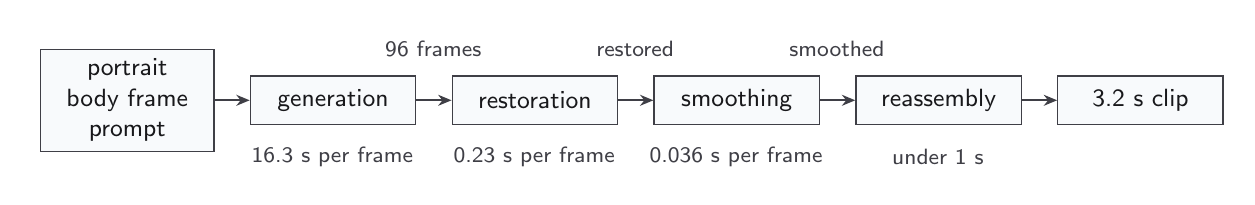
\begin{tikzpicture}
% bounding box: width = 433.34402pt = the deck text width; height as needed
\useasboundingbox (-0.0555cm,-0.9668cm) rectangle (-0.0555cm+433.34402pt,0.9223cm);
\fill[white] (-0.0555cm,-0.9668cm) rectangle (-0.0555cm+433.34402pt,0.9223cm);

% ---- one box for the three inputs, then the four stages and the clip --------
\node[proc,minimum width=2.2cm,anchor=west] (inp)  at (0.10,0) {portrait\\body frame\\prompt};
\node[proc,minimum width=2.1cm,anchor=west] (gen)  at (2.7636,0) {generation};
\node[proc,minimum width=2.1cm,anchor=west] (res)  at (5.3273,0) {restoration};
\node[proc,minimum width=2.1cm,anchor=west] (smo)  at (7.8909,0) {smoothing};
\node[proc,minimum width=2.1cm,anchor=west] (rea)  at (10.4546,0) {reassembly};
\node[proc,minimum width=2.1cm,anchor=west] (clip) at (13.0182,0) {3.2 s clip};

% ---- the flow --------------------------------------------------------------
\draw[fl] (inp) -- (gen);
\draw[fl] (gen) -- (res);
\draw[fl] (res) -- (smo);
\draw[fl] (smo) -- (rea);
\draw[fl] (rea) -- (clip);

% ---- what travels between the stages ---------------------------------------
\node[sub] at (5.0955,0.66) {96 frames};
\node[sub] at (7.6591,0.66) {restored};
\node[sub] at (10.2228,0.66) {smoothed};

% ---- cost of each stage ----------------------------------------------------
\node[sub] at (3.8136,-0.72) {16.3 s per frame};
\node[sub] at (6.3773,-0.72) {0.23 s per frame};
\node[sub] at (8.9409,-0.72) {0.036 s per frame};
\node[sub] at (11.5046,-0.72) {under 1 s};
\end{tikzpicture}
\end{document}
